\documentclass[times, twoside, watermark]{zHenriquesLab-StyleBioRxiv}
\usepackage{blindtext}
\usepackage{lipsum}
% Please give the surname of the lead author for the running footer
\leadauthor{Jane Doe} 

\begin{document}

% insert title
\title{Our very clever MIDOG 2022 contribution}
% insert title for footer
\shorttitle{Approach for MIDOG 2022}

% Use letters for affiliations, numbers to show equal authorship (if applicable) and to indicate the corresponding author
\author[1]{Jane Doe}
\author[2]{John Doe}
\author[1]{Jane Doe Sr.}

\affil[1]{School of Learning, University of Springfield, USA}
\affil[2]{Department of Machine Learning, TU Neustadt, Germany}

\maketitle

%TC:break Abstract
%the command above serves to have a word count for the abstract
\begin{abstract}
This is the abstract of your short paper describing your method contribution to the MIDOG 2022 MICCAI challenge. Make sure to summarize your contributions as well as your results in brief to help others and your reviewers to better understand your ideas and approaches. Please also make sure that you refer to the MIDOG 2022 challenge in title or abstract, so people know what this work is about.

\lipsum[5]
\end {abstract}
%TC:break main
%the command above serves to have a word count for the abstract

\begin{keywords}
keyword 1 | keyword 2 | keyword 3
\end{keywords}

\begin{corrauthor}
jane.doe@springfield.edu
\end{corrauthor}

\section*{Introduction}
This is your introduction. Please make sure you properly reference the challenge's formal description \cite{midog2022}. We appreciate if you also reference the overview paper of last year \cite{midog2021}, but it's not mandatory.

Figure \ref{fig:computerNo} shows an example of how to insert a column-wide figure. To insert a figure wider than one column, please use the \verb|\begin{figure*}...\end{figure*}| environment. Figures wider than one column should be sized to 11.4 cm or 17.8 cm wide. Use \verb|\begin{SCfigure*}...\end{SCfigure*}| for a wide figure with side captions.


\lipsum[2-5]

\section*{Material and Methods}

\lipsum[2-7]


\section*{Results}

\lipsum[2-2]

\begin{figure}%[tbhp]
\centering
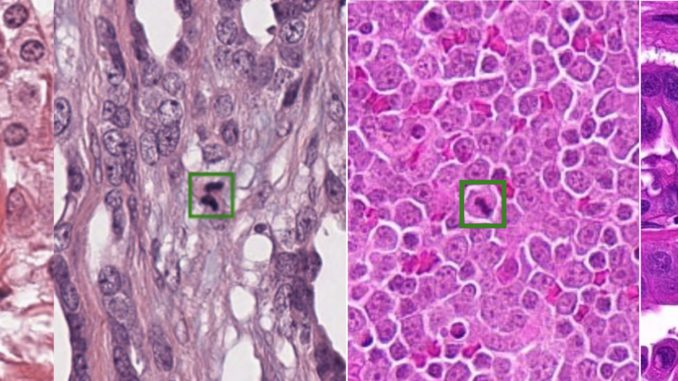
\includegraphics[width=\linewidth]{Figures/mitosis}
\caption{Placeholder image.}
\label{fig:computerNo}
\end{figure}

\lipsum[20]


\section*{Discussion}

\lipsum[20]

\begin{acknowledgements}
I thank the academy for this award.
\end{acknowledgements}

\section*{Bibliography}
\bibliography{literature}

\end{document}
